\lab{Algorithms}{Poisson's equation}{Poisson's equation}
\label{lab:finitedifference2}

 % The basic idea behind finite difference methods is to replace a 
 % differential operator, defined on some space of continuous functions, with a 
 % difference operator defined on a finite vector space (i.e., a space of grid functions).
 % 
 % To do this, we replace derivative terms in the differential equation with 
 % appropriate difference expressions. 
 % 
 % \begin{align*}
 % 	u_{xx}(t,x) &\approx \frac{(u(t,x+h)- 2u(t,x) + u(t,x-h))}{h^2},\\
 % 	u_x(t,x) & \approx \frac{u(t,x+h)-u(t,x-h)}{2h}.
 % \end{align*}
% Recall that the heat equation is given by $u_t = u_{xx} + f(x,t,u)$. 
Suppose that we want to describe the distribution of heat throughout a region $\Omega$.
Let $g(x)$ represent the temperature on the boundary of $\Omega$ ($\partial \Omega$), and let $h(x)$ represent the initial heat distribution at time $t = 0$.
If we let $f(x,t)$ represent any heat sources/sinks in $\Omega$, then the flow of heat can be described by the boundary value problem (BVP)
\begin{align}
	\begin{split}
		& { } u_t = \triangle u + f(x,t), \quad x \in \Omega, \quad t >0,\\
		& { }u(x,t) = h(x), \quad x \in \partial \Omega, \\
		& { }u(x,0) = g(x).
	\end{split}
\end{align}
When the source term $f$ does not depend on time, there is often a steady-state heat distribution $u_{\infty}$ that is approached as $t \to \infty$.
This steady state $u_{\infty}$ is a solution of the BVP
\begin{align}
	\begin{split}
		& { }  \triangle u + f(x) = 0, \quad x \in \Omega,\\
		& { }u(x,t) = h(x), \quad x \in \partial \Omega.
	\end{split}
\end{align}

This last partial differential equation, $\triangle u = -f$, is called Poisson's equation.
This equation is satisfied by the steady-state solutions of many other evolutionary processes.
Poisson's equation is often used in electrostatics, image processing, surface reconstruction, computational fluid dynamics, and other areas. 

\section{Poisson's equation in one dimension}
The 1D Poisson equation is given by 
\begin{align}
	\begin{split}
u'' &= f(x), \quad a \leq x \leq b,\\
	u(a) &= \alpha,\quad u(b) = \beta,
	\end{split} \label{eqn:1d_poisson}
\end{align}
where $f$ is continuous.
We will develop a finite difference method for solving this BVP. 

The basic idea behind most numerical methods for differential equations is to approximate the exact solution $u(x)$ at some finite collection of points in the 
domain of the problem.
Instead of analytically solving an infinite-dimensional problem, we look for a simple finite collection of algebraic equations that approximate the original problem.

Note that this equation can easily be solved by integrating twice and using the boundary conditions to determine the constants of integration.
Solving this \eqref{eqn:1d_poisson} is equivalent to solving the equation $\triangle u = f,$ where $\triangle = \frac{d^2}{dx^2}$ is a differential operator defined on the infinite-dimensional space of functions $u:[a,b] \to \mathbb{R}$ that are twice continuously differentiable and satisfy the boundary conditions $u(a) = \alpha$, $u(b) = \beta$.
The finite difference method replaces infinite-dimensional differential operators with finite-dimensional difference operators.

We consider an approximate solution $\{U_i\}_{i=-1}^N$ on an evenly spaced grid of $N$ subintervals, $a = x_{-1}, x_0, \ldots, x_{N-1} = b$ with $h = x_{i+1}-x_i$ for each $i$.
Recalling that $\frac{d^2}{dx^2}u(x) = \frac{1}{h^2}\left(u(x-h) -2u(x) + u(x+h)\right) + \mathcal{O}(h^2),$ we define the finite difference operator $D$ by  $DU_i = \frac{1}{h^2}\left(U_{i-1} -2U_i + U_{i+1}\right)$.
We may discretize \eqref{eqn:1d_poisson} using the equations 
\begin{align*}
	\frac{1}{h^2} (U_{i+1}- 2U_i + U_{i-1})  &= f(x_i), \quad i = 0, \ldots, N-2,
\end{align*}
along with boundary conditions $U_{-1} = \alpha,$ $U_{N-1} = \beta$.
This gives $N+1$ equations and $N+1$ unknowns, and can be written in matrix form as 
\[ \frac{1}{h^2} \begin{bmatrix}h^2 & 0 &0&\hdots &0 \\ 1 &-2 & 1 &\hdots &0\\ \vdots &  & \ddots & &\vdots \\
0 & \hdots & 1 & -2 & 1 \\ 0 & \hdots & & 0 & h^2
\end{bmatrix} \cdot \begin{bmatrix}U_{-1}\\U_0\\ \vdots \\U_{N-2} \\U_{N-1}\end{bmatrix} = \begin{bmatrix}f(x_{-1})\\f(x_0)\\ \vdots \\ f(x_{N-2}) \\ f(x_{N-1}) \end{bmatrix}\]
We can further modify the system to obtain an $(N-1)\times (N-1)$ tridiagonal matrix on the left: 
\[\frac{1}{h^2} \begin{bmatrix}-2 & 1 &0 & \hdots &0\\ 1 &-2 & 1 &\hdots &0\\ \vdots &  & \ddots & &\vdots \\ 0 & \hdots & 1 & -2 & 1 \\
0 & \hdots & 0 & 1 & -2 
\end{bmatrix} \cdot \begin{bmatrix}U_0\\U_1\\ \vdots \\U_{N-3}\\U_{N-2}\end{bmatrix} = \begin{bmatrix}f(x_0) -\alpha/h^2 \\f(x_1)\\ \vdots \\ f(x_{N-3})\\ f(x_{N-2})-\beta/h^2 \end{bmatrix}\]

The following code uses this finite difference method to solve the BVP
\begin{align*}
u'' &= -3 \sin{x}, \quad 0 \leq x \leq 2,\\
	u(0) &= -2,\quad u(2) = 1
\end{align*}

\begin{lstlisting}
import numpy as np
from scipy.sparse import spdiags
from scipy.sparse.linalg import spsolve

def bvp(func, a, b, alpha, beta, N):
    """ Solving u'' = f(x), x in [a, b],
    u(a) = alpha, u(b) = beta
    N = number of subintervals """
    
    # We use the finite difference method to construct a system 
    # of algebraic equations described by the matrix equation 
    # AU = F
    
    # The length of each subinterval
    h = (b - a) / N
    
    # Initialize and define the vector F on the right.
    F = np.empty(N - 1)
    F[0] = func(a + 1. * h) - alpha * h**(-2.)
    F[N-2] = func(a + (N-1) * h) - beta * h**(-2.)
    for j in xrange(1,  N-2): 
        F[j] = func(a + (j+1) * h)

    # Here we define the arrays that will go on the diagonals of A.
    data = np.empty((3, N-1))
    # main diagonal
    data[0,:] = -2. * np.ones((1, N-1))
    # off-diagonals
    data[1,:], data[2,:] = np.ones((1, N-1)), np.ones((1, N-1))
    # Next we specify on which diagonals they will be placed
    diags = np.array([0, -1, 1])
    
    A = h**(-2.) * spdiags(data, diags, N-1, N-1).asformat('csr')
    
    # We create and return the numerical approximation
    U = np.empty(N + 1)
    U[1:-1] = spsolve(A, F)
    U[0], U[-1] = alpha, beta
    return np.linspace(a, b, N+1), U

x, y = bvp(lambda x:(-3. * np.sin(x)), a=0., b=2., alpha=-2., beta=1, N=30)
\end{lstlisting}

\begin{comment}

How do we know if a numerical approximation is reasonable?
One way to determine this is to compute solutions for various step sizes $h$ and see if the solutions are converging to something.
To be more specific, suppose our finite difference method is $\mathcal{O}(h^p)$ accurate.
This means that the error $E(h) \approx Ch^p$ for some constant $C$ as $h \to 0$ (i.e., for $h>0$ small enough).
 
So compute the approximation $y_k$ for each stepsize $h_k$, $h_1 > h_2> \ldots>h_m$.
We will think of $y_m$ as the true solution.
Then the error of the approximation for 
stepsize $h_k, k < m,$ is 
\begin{align*}
	E(h_k) &= \max( \abs{ y_k - y_m}) \approx C h_k^p ,\\
	\log(E(h_k)) &= \log(C) + p \log(h_k).
\end{align*}
Thus on a log-log plot of $E(h)$ vs. $h,$ these values should be on a straight line with slope $p$ when $h$ is small enough to start getting convergence. 

The following code generates the log-log plot in \ref{figure1}, and demonstrates second-order convergence for this finite difference approximation. 
\begin{lstlisting}
import matplotlib.pyplot as plt
a, b = 0., 1.
num_approx = 10 # Number of Approximations
N = np.array([5*2**j for j in range(num_approx)])
h, max_error = (b-a)/N[:-1], np.ones(num_approx-1)

mesh_best, num_sol_best = bvp(lambda x:-3.*np.sin(x), a, b, alpha=-2., beta=1, N=N[-1])
for j in range(len(N)-1): 
    mesh, num_sol = bvp(lambda x:-3.*np.sin(x), a, b, alpha=-2., beta=1, N=N[j])
    max_error[j] = np.max(np.abs( num_sol- num_sol_best[::2**(num_approx-j-1)] ) )
plt.loglog(h,max_error,'.-r',label="$E(h)$")
plt.loglog(h,h**(2.),'-k',label="$h^{\, 2}$")
plt.xlabel("$h$")
plt.legend(loc='best')
plt.show()
print "The order of the finite difference approximation is about ", ( (np.log(max_error[0]) - 
    np.log(max_error[-1]) )/( np.log(h[0]) - np.log(h[-1]) ) ), "."
\end{lstlisting}

\begin{figure}[ht]
\centering
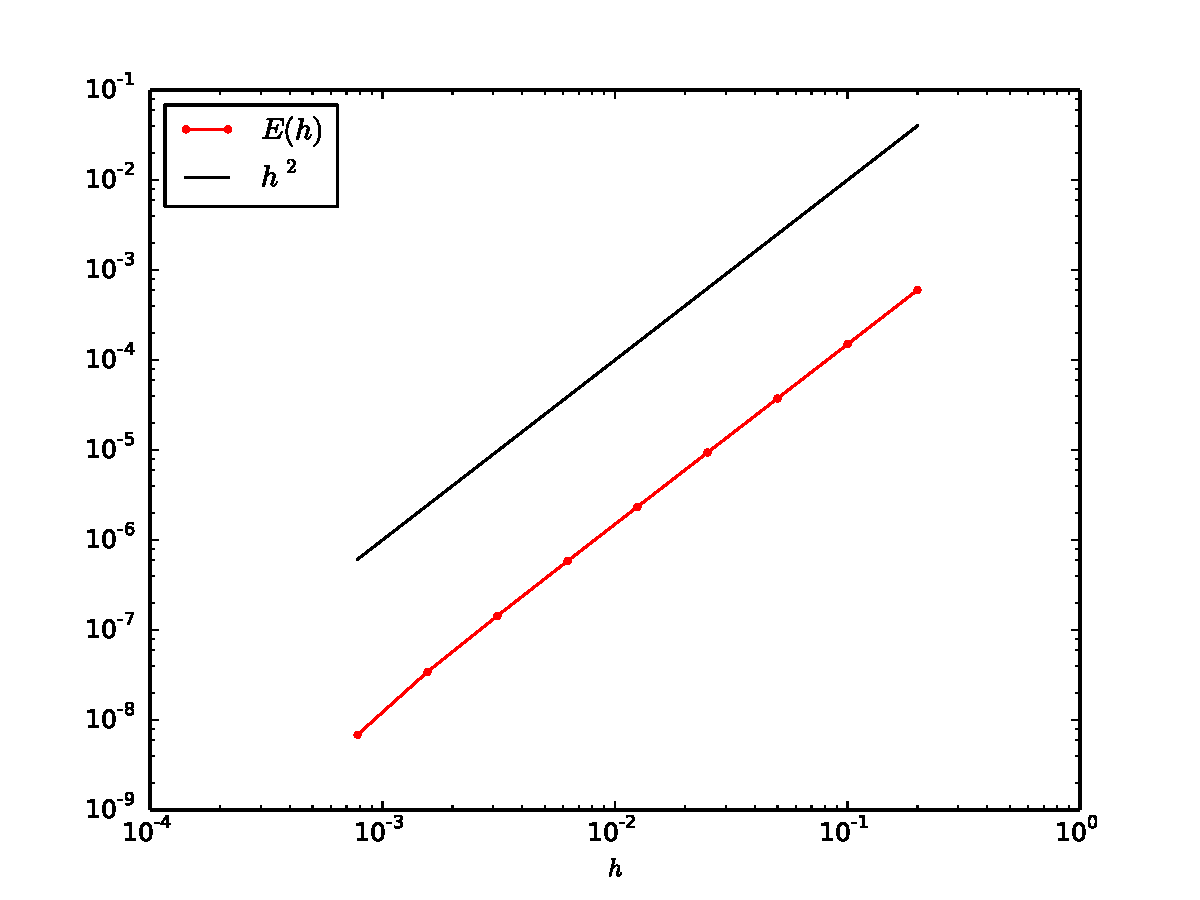
\includegraphics[width=12cm]{example_convergence.pdf}
\caption{TODO}
\end{figure}

\end{comment}

\begin{problem}
Extend the given finite difference code to the case of a general second order linear BVP with Dirichlet conditions:
\begin{align*}
	&{ } a_1(x)y'' +a_2(x)y'+ a_3(x) y = f(x), \quad x \in (a,b),\\
	&{ } y(a) = \alpha, \quad y(b) = \beta.
\end{align*}
Use your code to solve the singularly perturbed BVP
\begin{align}
	\begin{split}
	&{ } \epsilon y''(x)-y'= -1, \quad x \in (0,1), \\
	&{ } y(0) = 1, \quad y(1) = 3,
	\end{split} \label{eqn:singular_perturbed_BVP}
\end{align}
with $\epsilon = 1/10$.
How many subintervals are needed to obtain 4 digits of accuracy?

Hint: consider using a centered, forward, or backward differencing scheme to approximate $u'$.

% If $\alpha = 1$,  $\beta = 3$, and $f(x) = -1$, there is an exact solution: 
% \[y(x) = \alpha + x+ (\beta - \alpha -1)\frac{e^{x/\epsilon -1}}{e^{1/\epsilon -1}}\]
\end{problem}

\begin{figure}
\centering
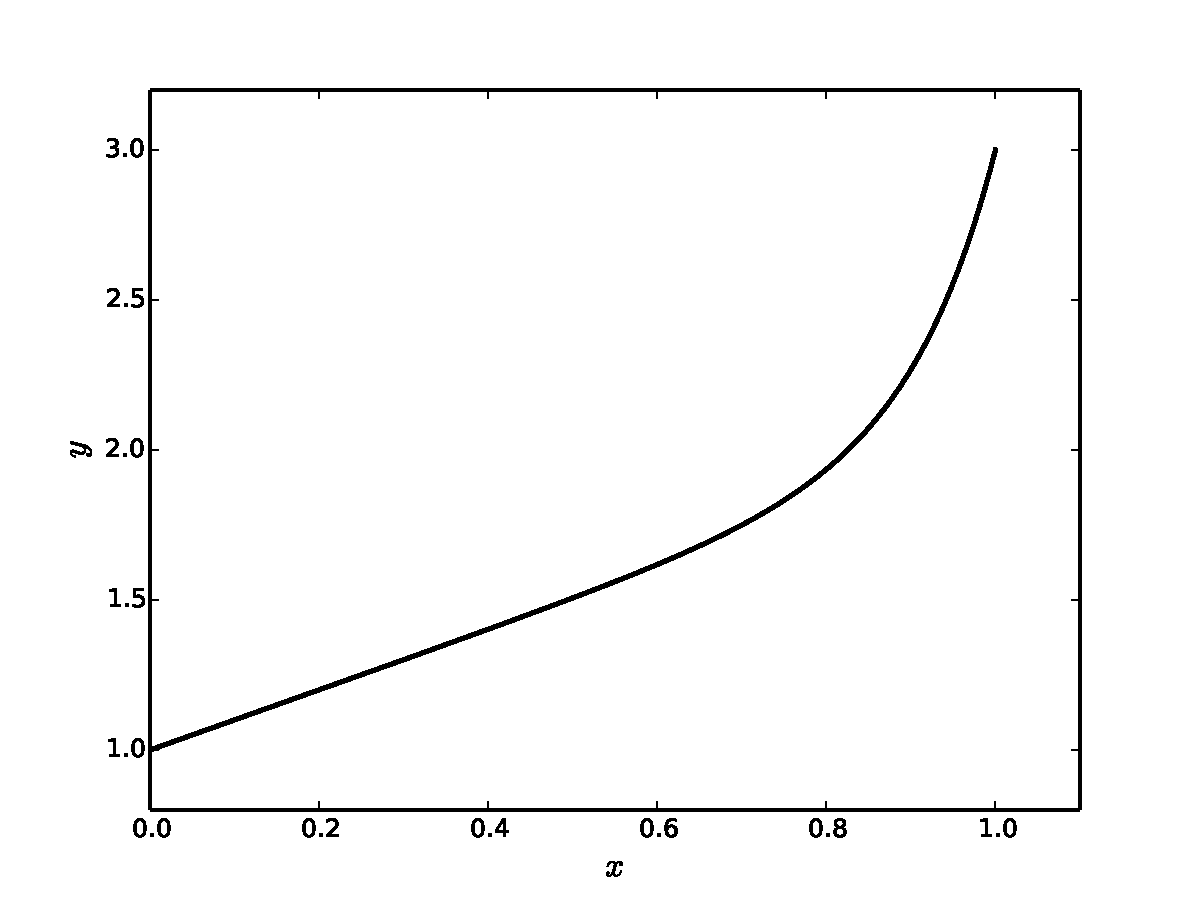
\includegraphics[width=12cm]{figure2.pdf}
\caption{The solution to \eqref{eqn:singular_perturbed_BVP}.
The solution gets steeper near $x = 1$ as $\epsilon $ gets small.}
\end{figure}

\section{Poisson's equation in two dimensions}

 Consider Poisson's equation together with Dirichlet boundary conditions on a rectangular  domain $R = [a,b] x [c,d]$:
 \begin{align}
	\begin{split}
 	u_{xx} + u_{yy} &= f,\quad x \text{ in } R \subset \mathbb{R}^2,\\
 	u &= g, \quad x \text{ on } \partial R.
	\end{split}\label{eqn:2d_poisson}
 \end{align}
Let $a = x_{-1}, x_0, \ldots, x_{N-1} = b$ be a partition of $[a,b]$, and let $c = y_{-1}, y_0, \ldots, y_{N-1} = d$ be a partition of $[c,d]$.
Suppose that there are $N+1$ evenly spaced points, so that $N$ is the number of subintervals in each dimension, and $x_i, y_j$ are given by 
\begin{align*}
	x_i &= a + (i+1)\triangle x, \\
	y_j &= c + (j+1)\triangle y,
\end{align*}
for $i,j = 0, \ldots, N-2$, where $\triangle x = x_i-x_{i-1}, \triangle y = y_i-y_{i-1}$.
We look for an approximation $U_{i,\,j}$ on the grid $\{(x_i,u_j)\}_{i,j=-1}^{N-1}$.

Recall that 
 \begin{align*}
 \triangle u = u_{xx}(x,y) + u_{yy}(x,y) &= \frac{u(x+h,y) - 2u(x,y)+ u(x-h,y)}{h^2} \\
 & \qquad{}+ 
 \frac{u(x,y+h) - 2u(x,y)+ u(x,y-h)}{h^2} + \mathcal{O}(h^2).
 \end{align*}
 We replace $\triangle $ with the finite difference operator $\triangle_h$, defined by 
 \begin{align*}
 \triangle_h U_{ij} &= \frac{U_{i+1,\,j} - 2U_{i,\,j} + U_{i-1,\,j}}{h^2} + \frac{U_{i,\,j+1} - 2U_{i,\,j}+ U_{i,\,j-1}}{h^2},\\
&= \frac{1}{h^2}(U_{i-1,\,j} + U_{i+1,\,j} + U_{i,\,j-1} + U_{i,\,j+1}-4U_{i,\,j}).
 \end{align*}
 Then the set of equations  $\triangle_h U_{ij} = f_{ij}$, $i,j = 0,\ldots,N-2$ % $i,j = 1,\ldots,m$ 
can be written in matrix form as
 \[AU + p +  q  = \]

$A$ is a block tridiagonal matrix, given by 
\[\frac{1}{h^2}
\begin{bmatrix}
T & I & &  &\\
I &T & I & &\\
&\ddots  & \ddots & \ddots & \\
&  & I & T & I \\
&  &  & I & T\end{bmatrix}\]
where $I$ is the $N-1\times N-1$ % $m\times m$
identity matrix, and $T$ is the tridiagonal matrix
\[\begin{bmatrix}
-4 & 1 & &  &\\
1 &-4 & 1 & &\\
&\ddots  & \ddots & \ddots & \\
&  & 1 & -4 & 1 \\
&  &  & 1 & -4 \end{bmatrix}\]

The vector $U$ is given by 
\[U = \begin{bmatrix} U^0 \\ U^1 \\ \\ U^{N-2} \end{bmatrix} \text{ where } U^j = 
\begin{bmatrix} U_{0,\,j} \\ U_{1,\,j} \\ \\ U_{N-2,\,j} \end{bmatrix} \text{ for each } j, 0\leq j \leq N-2\]

% \[U = \begin{bmatrix} U^1 \\ U^2 \\ \\ U^m \end{bmatrix} \text{ where } U^j = 
% \begin{bmatrix} U_{1,\,j} \\ U_{2,\,j} \\ \\ U_{m,\,j} \end{bmatrix} \text{ for each } j, 1\leq j \leq m\]
% So $U^j$ represents the $j$th row of interior points in our grid, where $y_j = jh$

The vectors $p$ and $q$ come from the boundary conditions of \eqref{eqn:2d_poisson}, and are given by 
\[p = \begin{bmatrix} p^0 \\ \ldots \\ \\ p^{N-2} \end{bmatrix}, \quad  q = \begin{bmatrix} q^0 \\ \ldots \\ \\ q^{N-2} \end{bmatrix}\]
where 
\[p^j = \frac{1}{h^2} \begin{bmatrix} g_{-1,\,j} \\ 0 \\ \vdots \\0\\ g_{N-1,\,j} \end{bmatrix} ,\,\,\, 0 \leq j \leq N-2\]
and 
\[q^0 = \frac{1}{h^2}\begin{bmatrix} g_{0,-1}  \\ g_{1,-1} \\ \vdots \\ g_{N-3,-1}\\ g_{N-2,-1} \end{bmatrix}, \quad q^{N-2} = \frac{1}{h^2}\begin{bmatrix} g_{0,N-1} \\ g_{1,N-1} \\ \vdots \\ g_{N-3,N-1}\\ g_{N-2,N-1} \end{bmatrix}, \quad q^{j} = \begin{bmatrix} 0 \\ 0 \\ \vdots \\ 0 \\ 0 \end{bmatrix} ,\,\,\, 1 \leq j \leq N-3\]

% The vector $q$ is given by $u = [q^0 \ldots q^{N-2}]^T$, %   $u = [q^1 \ldots q^m]^T$,
% where 
% \[q^j = \frac{1}{h^2} \begin{bmatrix} g_{0,\,j} \\ 0 \\ \vdots \\0\\ g_{m+1,\,j} \end{bmatrix} , \,\,\, 2 \leq j \leq m-1\]
% and 
% \[q^1 = \frac{1}{h^2}\begin{bmatrix} g_{1,0} + g_{0,1} \\ g_{2,0} \\ \vdots \\ g_{m-1,0}\\ g_{m,0} + g_{m+1,1}\end{bmatrix}, \quad q^m = \frac{1}{h^2}\begin{bmatrix} g_{1,m+1} + g_{0,m}\\ g_{2,m+1} \\ \vdots \\ g_{m-1,m+1}\\ g_{m,m+1} + g_{m+1,m}\end{bmatrix}\]

% \begin{problem}
% Find the solution $u$ of the 2D Laplace equation $\Delta u = 0$ on the unit 
% square $[0,1]\times [0,1] \subset \mathbb{R}^2,$ subject to the (Dirichlet) condition that 
% $u(x,y) = x^3$ on the boundary. 
% 	 
% Graph your solution, and demonstrate convergence of the numerical approximation by 
% creating a log-log plotof the error $E(h).$
% \end{problem}

% \begin{problem}
% Find the solution $u$ of the 2D Poisson equation with the given Dirichlet boundary conditions:
% \begin{align*}
% 	\Delta u &= -\pi^2 \sin(\pi x)\sin(\pi y), \quad (x,y) \in [0,1]\times [0,1], \\
% 	u(x,0) &= 1-x, \\
% 	u(x,1) &= 1-2x, \\
% 	u(0,y) &= 1, \\
% 	u(1,y) &= -y. 
% \end{align*}
% 
% Graph your solution, and demonstrate convergence of the numerical approximation by 
% creating a log-log plot of the error $E(h).$
% \end{problem}

% The matrix $A$ is sparse, and so we can use several functions from the package \texttt{scipy.sparse.linalg}.
% In particular, we use the functions \texttt{spdiags} and \texttt{spsolve}.
%  
%  \begin{verbatim}
% D1,D2,D3 = -4*np.ones((1,m**2)), np.ones((1,m**2)), np.ones((1,m**2)) 
% Dm1, Dm2 = np.ones((1,m**2)), np.ones((1,m**2))
% for j in range(0,D2.shape[1]):
% 	if (j%m)==m-1: 
% 		D2[0,j]=0
% 	if (j%m)==0: 
% 		D3[0,j]=0
% diags = np.array([0,-1,1,-m,m])
% data = np.concatenate((D1,D2,D3,Dm1,Dm2),axis=0) # This stacks up rows
% A = 1./h**2.*spdiags(data, diags, m**2,m**2).asformat('csr') # This ap
%  \end{verbatim}
 
\begin{comment}
\subsection{2D Heat Equation}
Recall that the collection of finite difference equations
\[\nabla^2_h U_{ij} = 0, \quad 1 \leq i,j\leq m\]
can be written in matrix form as
\[AU + q  = 0\]

The Crank-Nicolson method for the 2D heat equation is given by 
\[U_{i,\,j}^{n+1}- U_{i,\,j}^{n} = \frac{\Delta t}{2}(\nabla_h^2 U_{i,\,j}^{n} + \nabla_h^2 U_{i,\,j}^{n+1}) \text{ for each } 1 \leq i,j \leq m\]
is a second order accurate in both space and time. Basically we're using a midpoint scheme in time, 
and a trapezoidal scheme in space. The resulting method is implicit, and can be written in matrix form as 
\begin{align*}
	IU^{n+1} &= IU^n + \frac{\Delta t}{2}(AU^n + q + AU^{n+1} + q)\\
	(I - \frac{\Delta t}{2}A)U^{n+1}&= (I + \frac{\Delta t}{2}A)U^n + \Delta t q
\end{align*}

% TODO: What size must the time step be to ensure stability? 

We will need to take many time steps, where many equations must be solved with the matrix $(I - \frac{\Delta t}{2}A)$.
The function \texttt{factorized} from \texttt{scipy.sparse.linalg} computes the LU decomposition of the matrix.
This decomposition reduces the time required for solving consecutive time steps.
\end{comment}

\section{Poisson's Equation and Conservative Forces}
In physics Poisson's equation is used to describe the scalar potential of a conservative force (we'll explain what each of these terms mean).
A conservative force $\bold{F}(\bold{r})$ is a vector function that obeys any of three equivalent conditions
\begin{enumerate}
	\item The curl is identically zero
		\[\nabla \times \bold{F}(\bold{r}) = 0\]
	\item It can be written as the negative of a gradient, called the scalar potential
		\[\bold{F}(\bold{r}) = - \nabla U(\bold{r})\]
	\item The line integral over a closed path is zero
		\[\oint \bold{F}(\bold{r}) \cdot d\bold{r} = 0\]

\end{enumerate}
\textit{Note: Letters in bold are vector quantities}

The scalar potential defined over the space is a measure of the potential energy a particle would have if placed at that point.
It could be electric potential energy, gravitational potential energy, or anything else governed by a conservative force.

Whenever we have a conservative force we can use a few identities from vector calculus to obtain Poisson's equation for it's scalar potential. 
Consider for example the electrostatic force, the force that two electric charges exert on each other. 
It can be summarized in two of Maxwell's four equations.
\[\nabla \times \bold{E} = -\frac{\delta \bold{B} } {\delta t} \qquad
\nabla \cdot \bold{E} = \frac{\rho}{\epsilon_0}\]
Where $\bold{E}$ is the electric field, $\bold{B}$ is the magnetic field, $\rho$ the charge density, and $\epsilon_0$ the permisivity of free space, a constant. $\nabla \times$ and $\nabla \cdot$ represent respectively the curl and the divergence operators. In the absence of a changing magnetic field the curl is zero and so we have a conservative force (although $\bold{E}$ is not actually a force but a force per charge we can still treat it as a conservative field, proportionaly to a related conservative force). Because the curl is zero we can immediately assume the other properties of a conservative force and write $\bold{E}$ as a gradient
\[\bold{E}  = - \nabla V = 0\]
$V$ is called the electrostatic scalar potential, more commonly known as the voltage. 
If we insert this into the equation for the divergence of $E$ we find after the application of the identity $\nabla \cdot (\nabla\psi) = \Delta \psi$
\[\nabla \cdot ( - \nabla V) = - \Delta V = \frac {\rho}{\epsilon_0}\]
With this we have Poisson's equation for electrostatics. 
If there are no charges ( or that the divergence of $E$ is zero), then this reduces to Laplace's equation. 
A similar analysis can be applied using Gauss's law of gravity (a reformulation of Newton's law of gravity in terms of a divergence) for a description of the gravitational scalar potential in terms of mass density.

Unfortunately, because in most physical systems charges are free to roam, this electric potential feeds back into the system and changes the charge distribution. 
This means that in reality $V$ is present on both sides of the equation.
In fact it is usually non-linear. 
However, in the following analysis, we'll assume that the charges are fixed in space, or "frozen in".
We'll also ignore all constants (specifically $\epsilon_0$) and units so that we are really dealing with the relative charge.

One simple application of the electric potential is to calculate basic properties of simple molecules, starting from a charge distibution and from that calculating the electric potential field.
We'll assume that the electrons produce a clouds of charge centered around the atoms, appoximated by a Boltzmann Distribution $\rho = q e^{-r}$, where $q$ is the relative charge of the atom and $r$ is the distance from the atom. 
To make this easier, we'll make a function (\li{rho1}) to calculate the $\rho$ value at a certain point in space based the position of an atom and it's relative charge. 
We'll make another function (\li{rhoSum}) to give the total charge density at a point based on a list of atoms.

\begin{lstlisting}
#definitions for atoms position and charges
#the angle the hydrogen atoms make
theta = 106.0/180.0*np.pi
#Length of the two branches
A = 1.0
# Hydrogen 1 (x0,y0,q)
# Hydrogen 2 
# Oxygen
water = ((-np.sin(theta / 2) * A, 0, 1),
         (np.sin(theta / 2) * A, 0, 1),
         (0, -np.cos(theta / 2) * A, -2))

def rho1(x, y, atom):
    return atom[2] * np.exp(-np.sqrt((x - atom[0])**2 + (y - atom[1])**2))

def rhoSum(x,y,atoms):
    return np.sum([rho1(x,y,atom) for atom in atoms],axis=0)

# Generate a color dictionary for use with LinearSegmentedColormap.
# It places red and blue at the min and max values of data
# and white when data is zero.
def genDict(data):
    zero = 1 / (1 - np.max(data) / np.min(data))
    cdict = {'red':[(0.0,  1.0, 1.0),
                   	(zero,  1.0, 1.0),
                   	(1.0,  0.0, 0.0)],
         'green':  [(0.0,  0.0, 0.0),
                   	(zero,  1.0, 1.0),
                   	(1.0,  0.0, 0.0)],
         'blue':   [(0.0,  0.0, 0.0),
                   	(zero,  1.0, 1.0),
                   	(1.0,  1.0, 1.0)]}
    return cdict
X = np.linspace(-5, 5, 100)
X, Y = np.meshgrid(X, X)
# Generate the grid of rho values.
Rho = rhoSum(X, Y, water)
plt.imshow(Rho, cmap =  mcolors.LinearSegmentedColormap('cmap', genDict(Rho)))
plt.colorbar()
plt.show()
\end{lstlisting}
The function \li{genDict} scales the color values to be white when the charge density is zero.
This is mostly to help visualize where there are neutrally charged zones by forcing them to be white.
You may find it useful to also apply it when you solve for the electric  potential.

\begin{figure}
\centering
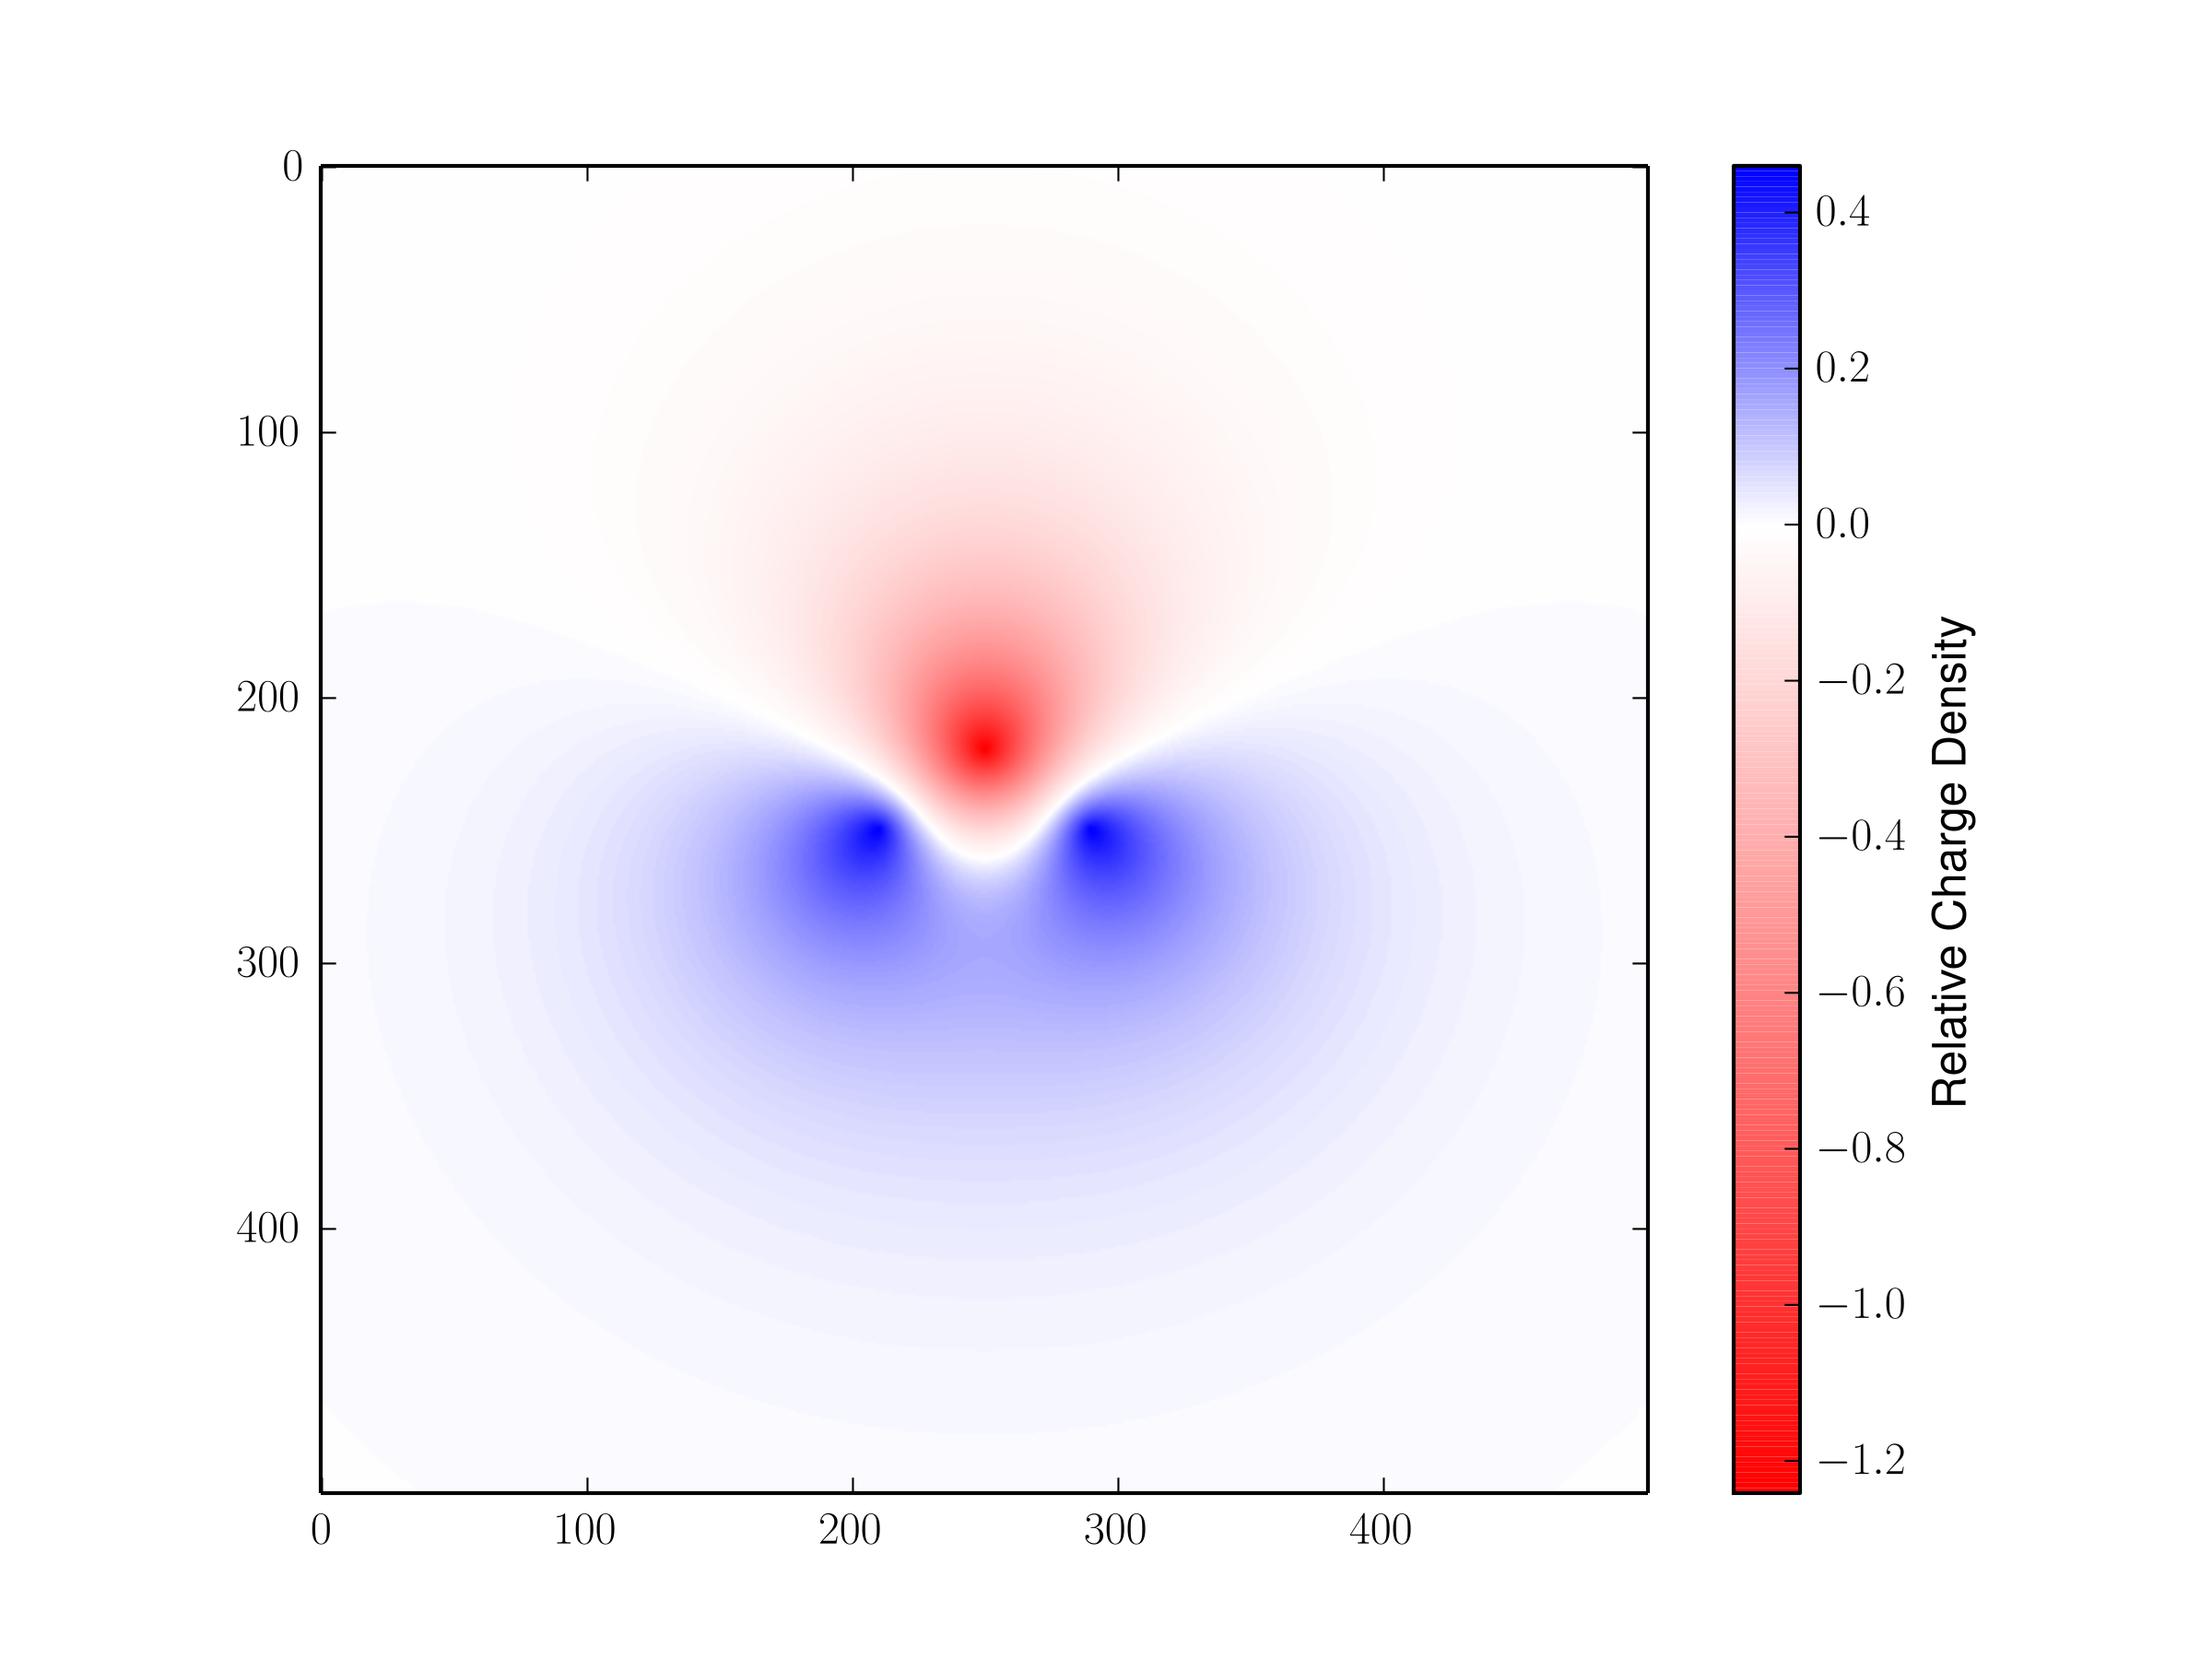
\includegraphics[width=12cm]{waterRho.png}
\caption{Relative charge density of an H$_2$O molecule}
\end{figure}

With a function for $\rho$, we can solve Poisson's equation for the electric potential field.
\begin{problem}
Solve for the electric potential $V$
\[\Delta V = -\rho(x,y)\]
The electric potential is usually defined to go to zero at inifinity.
We can approximate this using $V=0$ at the boundry conditions on $[-5,5]\times [-5,5]$.
Solve and plot the electric potential of water, using the definition for the atoms above.

\end{problem}

\begin{problem}
Solve for the electric potential of a CO$_2$ molecule.

CO$_2$ can be modeled as two atoms of relative charge $-1$ placed at $x=-1$ and $x=1$ on the $x$ axis and a third atom with relative charge $2$ at the origin.
Simply reuse your code from the last problem with new definitions for the atoms using the template for a water molecule.

If the molecules are moving slowly (ie. when the temperature is low) electrostatic forces will dominate molecular interactions.
Molecules will want to align themselves in the lowest energy configuration, or the lowest electric potential.
Positive potentials will overlap themselves with negative potentials.
From the electric potential plots you obtain, how do you think the molecules will arrange themselves when the temperature is cold, when they form an ice?
\end{problem}

\begin{figure}
\centering
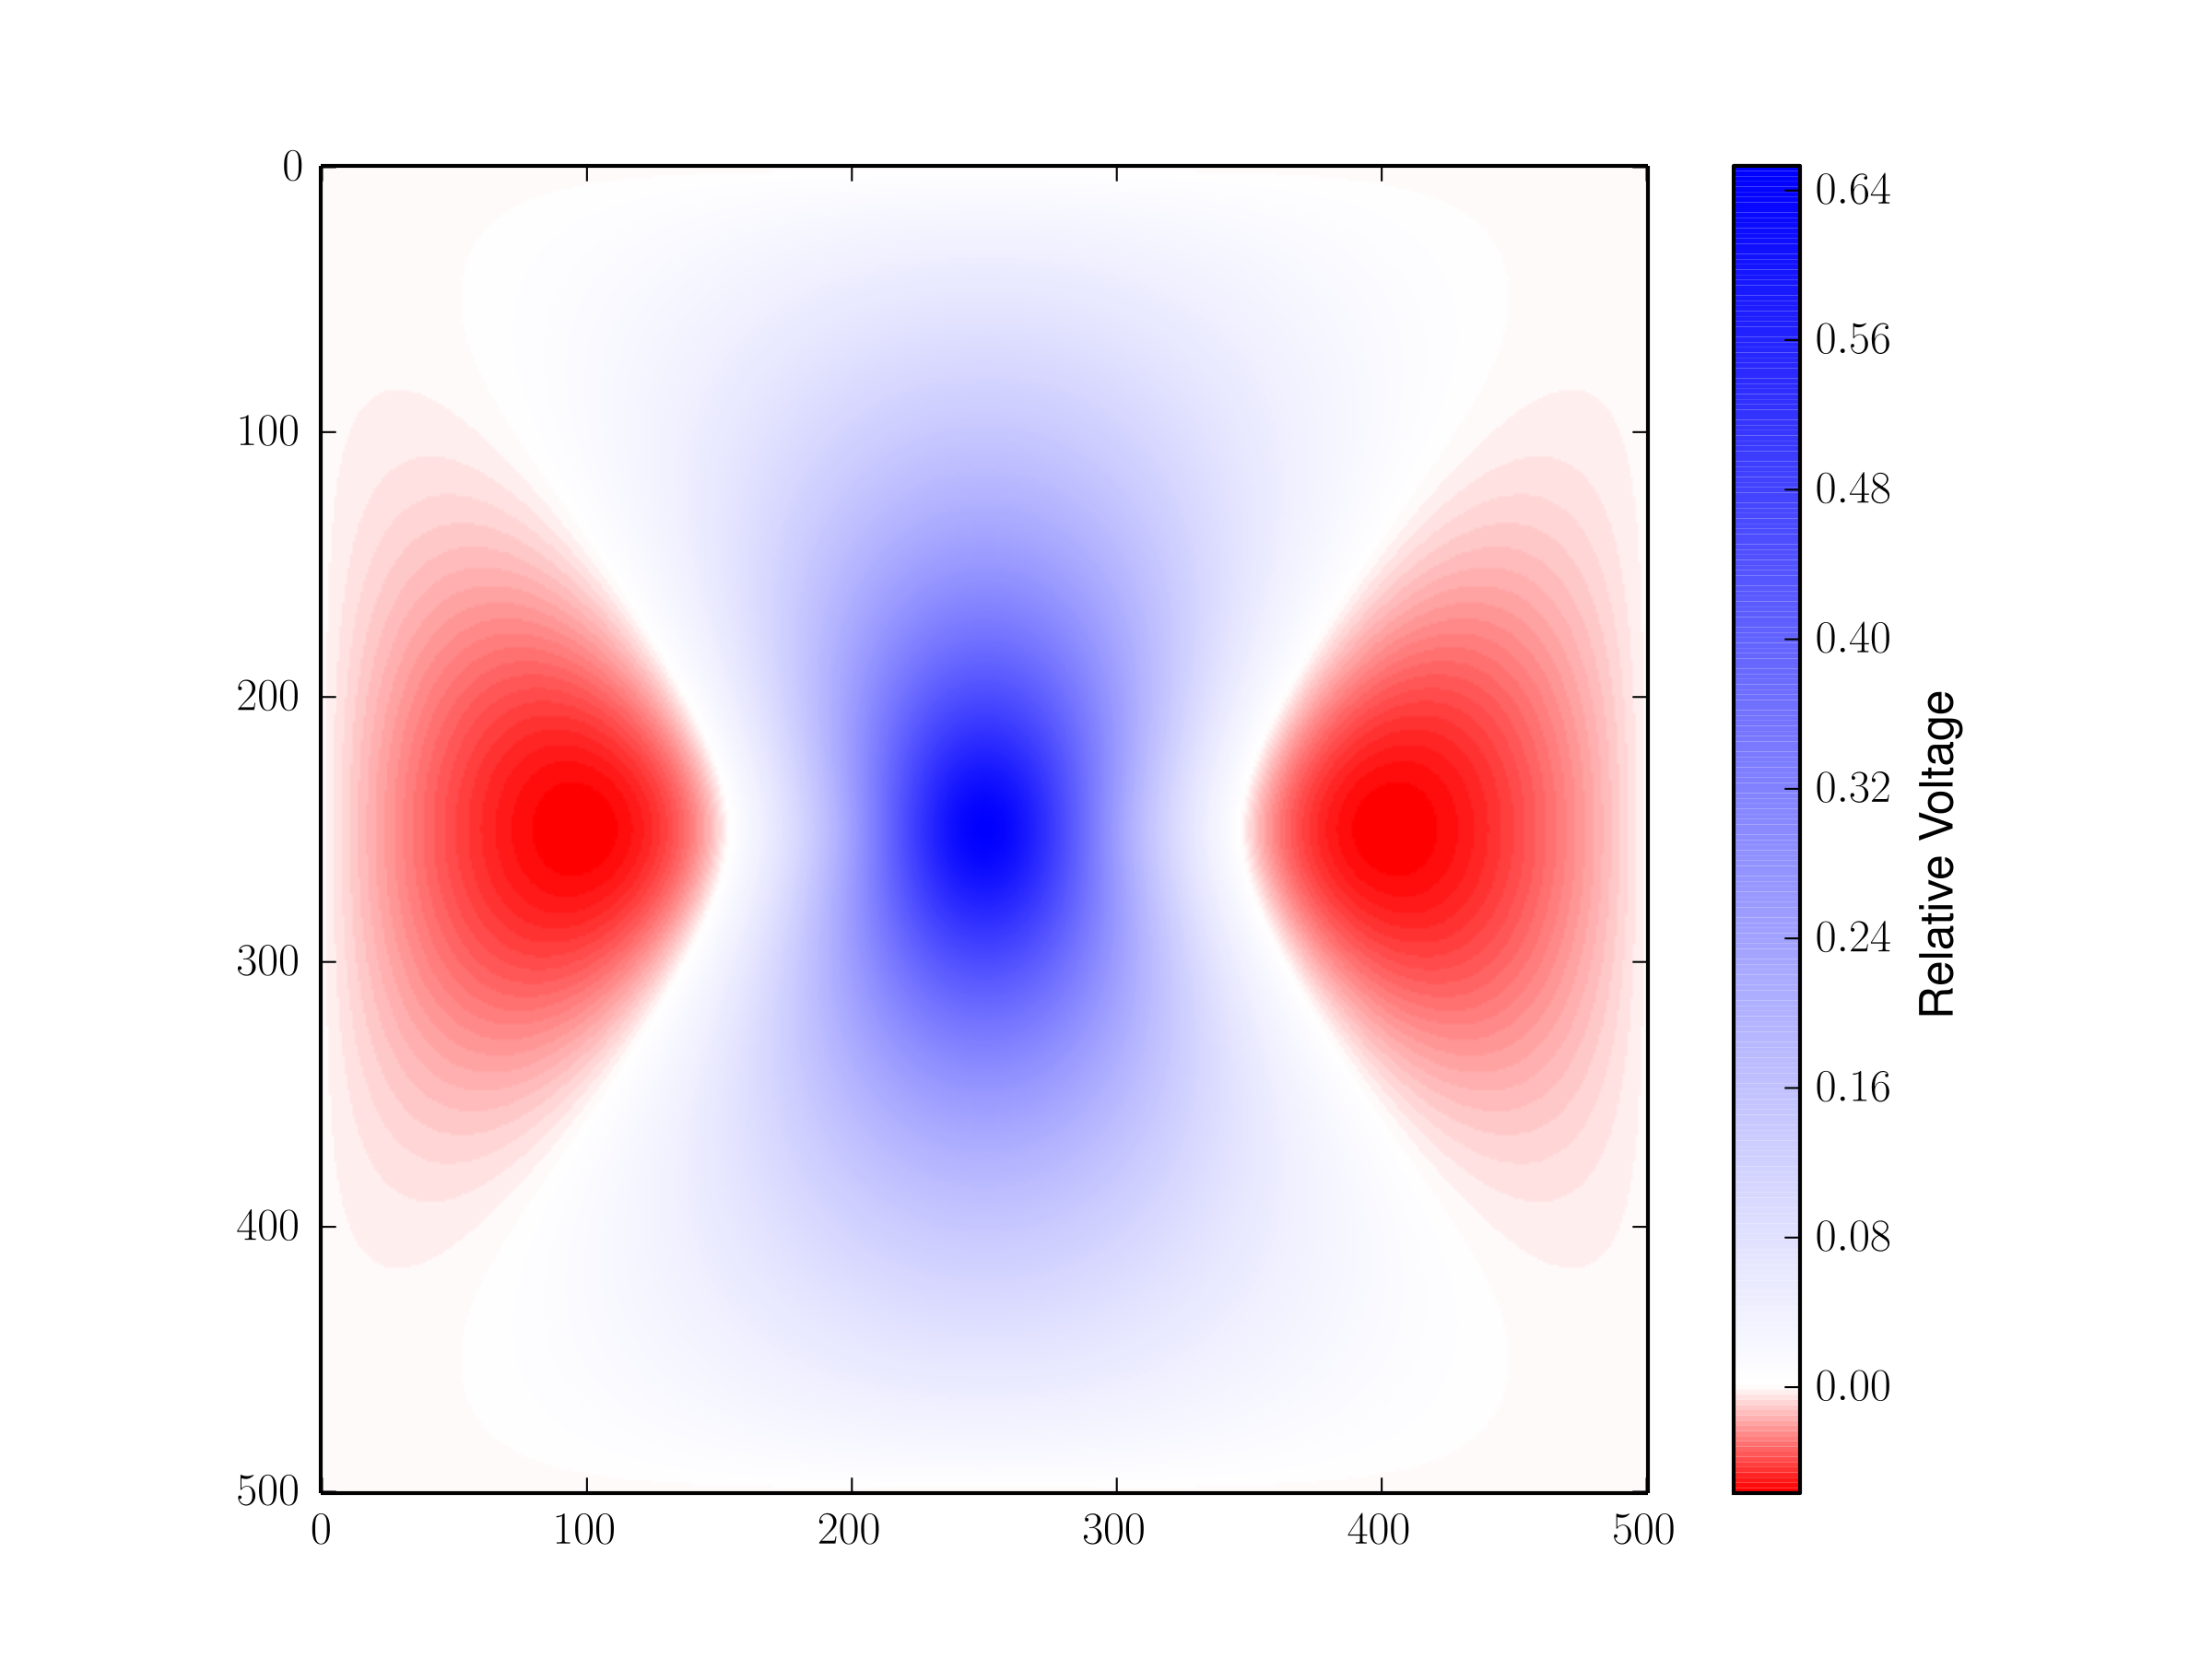
\includegraphics[width=12cm]{co2V.png}
\caption{Relative electric potential field of a CO$_2$ molecule}
\end{figure}